% !TeX spellcheck = cs_CZ
\begin{mdframed}[style=mdexam]
  \begin{example}\label{MAI:exam029}
  Nechť \(\varphi(x) = \sqrt[3]{x}\), \(a = 0\). Pak \(f(x) = \frac{\sqrt[3]{x}}{x}\). Pro \(x \neq
  0\) je \(f(x) = \frac{1}{\sqrt[3]{x^2}}\). Jestliže \(x \to 0\), pak hodnoty \(f(x)\) neomezeně
  vzrůstají, protože jmenovatel zlomku se blíží kladnými hodnotami k nule a čitatel je stále roven
  \(1\) (viz obr. \ref{mai:fig018}). Místo rčení „funkce neomezeně roste“ pro \(x \to 0\) říkáme též
  „funkce se blíží k \(+\infty\)“ pro \(x \to 0\) a píšeme \(lim_{x\to 0} f(x) = +\infty\) nebo
  \(f(x) \to +\infty\) pro \(x \to 0\). Říkáme, že limita funkce \(f\) v bodě \(0\) je rovna
  \(+\infty\). 
    
    {\centering
    \captionsetup{type=figure}
  %   \documentclass[11pt]{standalone}
\usepackage{xltxtra}
\usepackage[usenames,x11names]{xcolor}
\usepackage{tikz}
  \usetikzlibrary{intersections}
  \usetikzlibrary{decorations.markings}
\usepackage{pgfplots}
  \pgfplotsset{compat=newest}
  
\usepackage{amsmath}

\begin{document}
  \begin{tikzpicture}[thick,scale=0.7, 
      every node/.style={transform shape},
      ]
  
  \tikzset{->-/.style={decoration={
    markings,
    mark=at position #1 with {\arrow{stealth}}},postaction={decorate}}}
    
    \begin{axis}[
      xmin = -2.5, xmax = 2.5, ymin = 0, ymax = 3.5,  % osy
      domain = -1:3.5,
      restrict y to domain=0:3.4,
      axis equal image,
      grid = major,   % both
      grid style={line width=.1pt, draw=gray!20},
      major grid style={dashed, line width=.2pt, draw=gray!40},
      clip = true,
      clip mode=individual,
      xtick={-2,-1,1,2,3,4}, % make steps of length 0.2
      ytick={0,1,2,3,4,5}, 
      axis x line = middle,
      axis y line = middle,
      xlabel={\(x\)}, ylabel={\(y\)},
      enlarge y limits={rel=0.07},
      enlarge x limits={rel=0.07},
      ]
  
        \addplot[color=Gold3, samples=100, smooth, ultra thick, unbounded coords=jump,
                 no markers, domain = 0.1:2, name path global=func1] 
           gnuplot{1/((x^2.0)^(1/3.0))};
  
        \addplot[color=Gold3, samples=100, smooth, ultra thick, unbounded coords=jump,
                 no markers, domain = -2:-0.1, name path global=func2] 
           gnuplot{real(1/((x^2.0)^(1/3.0)))};
  
        \node [fill=white] at (rel axis cs: 0.75,0.5) {\(y=\dfrac{1}{\sqrt[3]{x^2}}\)};
  
        \path[name path=line] (-1,1.5) -- (1,1.5); 
            % Intersections points
            \path [name intersections={of=func1 and line,by={P1}}] (P1) node [] {};
  
        \path[name path=line] (-1,1.5) -- (1,1.5); 
            % Intersections points
            \path [name intersections={of=func2 and line,by={Q1}}] (Q1) node [] {};
        
        \draw[black,fill=black] (P1) circle (.3ex);
        \draw[black,fill=black] (Q1) circle (.3ex);
        \path (P1 |- 3,0) -- (P1) -- (P1 -| 0,3) node (X) {};
  
        \draw[thick,red, fill=white] ([shift=(0:1mm)]X) arc (0:180:1mm);
        \draw[->-=.5, dashed]  (P1 |- 3,-0.1)  
          node[below] {\(\delta\)} -- (P1) -- (P1 -| 0,3);
        \draw[->-=.5, dashed]  (Q1 |- -3,-0.1) 
          node[below] {\(\delta\)} -- (Q1) -- (Q1 -| 0,3);
  
        \draw[line width = 2pt, red, line cap=butt] (Q1 |- 3,0) -- (P1 |- 3,0);
        
        \path[name path=line] (-0.7,2.5) -- (0.7,2.5); 
            % Intersections points
            \path [name intersections={of=func1 and line,by={P1}}] (P1) node [] {};
            \draw[->-=.4, dashed, thin,gray] (P1 |- 3,-0.05) node[below] {\(x\)} -- (P1);
            \draw[->-=1, thin, gray] (P1) -- (P1 -| 0,3) node[left, fill=white] {\(f(x)\)};
        \draw[thick,red] (X) node[below left] {\(q\)} -- ++(0cm,2.5cm);
  
       \draw[black,fill=white] (0,0) node[below left] {\(O\)} circle (.4ex);
    \end{axis}
  \end{tikzpicture}
\end{document}
    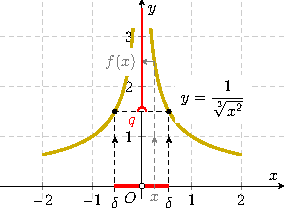
\includegraphics[width=0.8\linewidth]{mai_fig018.pdf}
    \captionof{figure}{K příkladu \ref{MAI:exam029}
    \cite[s.~118]{Brabec1989}
    \label{mai:fig018}}
    \par}
    
    Přesně to znamená toto: Zvolíme-li libovolně velké \(q > 0\), můžeme nalézt \(\delta > 0\) tak,
    že pro každé \(x \neq 0\), pro něž \(\abs{x} < \delta\), platí \(f(x) > q\). To lze říci i
    takto: Zvolíme-li libovolně okolí bodu \(+\infty\), existuje okolí bodu \(0\) tak, že pro každé
    \(x \neq 0\) z tohoto okolí je \(f(x)\) ve zvoleném okolí \(+\infty\) (viz obr.
    \ref{mai:fig018}).
  \end{example}
\end{mdframed}















